Táto kapitola priblíži, akým spôsobom budeme riešiť cieľe aplikácie definované v špecifikácii. Spomenie sa tu architektúra aplikácie, vzťahy medzi jednotlivými častami aplikácie, reprezentácia údajov a návrh riešenia konkrétnych problémov.\par
\section{Jazyk}
Našim programovacím jazykom pre ktorý sme sa rozhodli je jazyk Java. Jednou z najväčších výhod tohto jazyka je jeho univerzálnosť. Je prístupný na všetkých možných platformách a programátor sa nemusí zaoberať rodzielmi medzi platformami a kód bude funkčný. Ďaľšou výhodou je štrukturovateľnosť aplikácie v tomto jazyku. Túto výhodu využijeme naplno a povieme si o architektúre aplikácie v ďaľšej sekcii. Tento jazyk je objektovo orientovaný a teda pri architektúre si spomenieme aj aké objeky sa budú vyskytovať v našej aplikácii.
\section{Architektúra}
Pred implementáciou aplikácie je vhodné si rozvrhnúť architektúru aplikácie a definovať, čo bude každá z častí obsluhovať. Aplikáciu sme si rozdelili na tri časti a každá z týchto častí bude reprezentovaná balíčkom v Jave. Táto sekcia pojednáva čisto o architektúre aplikácie návrh riešenia jednotlivých problémov bude popísaný neskôr.\par
Prvá časť aplikácie bude obsluhovať načítavanie herných objektov z textových súborov. Bude sa venovať aj generovniu herného sveta pomocou načítaných objektov. Ďalej bude sprosdredkúvať generovanie akcií, ktoré sa budú využívať na plánovanie príbehu a samotné hranie hry. Taktiež zaistí zapisovanie reprezentácie herného sveta do súboru a aj jeho načítavanie zo súboru.\par
Druhá časť sa bude zaoberať definíciou reprezentácie akcie. Bude sa tu odohrávať aj plánovanie príbehu a následné ohodnocovanie zaujímavosti tohto príbehu.\par
Posledná časť bude obsluhovať samostatné hranie vygenerovaného príbehu. Tiež sa bude venovať komunikácii medzi používateľom a aplikáciou a prepojí ostatné dve časti aplikácie. Grafickú reprezentáciu vzťahov medzi spomínanými častami môžeme vidieť na obrázku 3.1.
\begin{figure}[H] 
\begin{center}
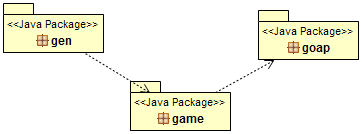
\includegraphics[scale=1.0]{img/packages.png}
\caption{Grafické reprezentácia Java balíčkov našej aplikácie.}
\label{fig:ch31}
\end{center}
\end{figure}
Na tomto obrázku balíček gen zahrňuje funkcionalitu generovania spolu s načítavaním a zapisovaním do súboru. Balíček goap v sebe skrýva funkcionalitu plánovania a reprezentáciu akcií. A posledný balíček game obsahuje samotnú hru a ovládanie aplikácie. Šípky naznačujú vzťahy medzi balíčkami, kde balíček gen pomocou jeho funkcií vygeneruje objekty do balíčka game a ten následne použije funkcie z balíčka goap na naplánovanie a ohodnotenie jeho príbehu a výsledok zobrazí používateľovi.
\subsection{Balíček gen}
Tento balíček bude obsahovať triedy zabezpečujúce načítavanie herných objektov, generovanie herného sveta a akcií a aj zapisovanie herného sveta do súboru. Mal by teda obsahovať tri triedy, z toho každá bude obsluhovať vyššie uvedené funkcionality.\par
Prvá trieda bude FileLoader, ktorá zabezpečí prácu so súborom. V tejto triede by sa mali nachádzať štyri funkcie, ktoré obslúžia všetkú interakciu so súbormi v našej aplikácii. Ďaľšou v poradí bude trieda WorldGenerator, ktorá bude mať na starosti generovanie herného sveta za pomoci objektov, ktoré načítal FileLoader. Na koniec v tomto balíčku budeme mať triedu ActionGenerator, ktorá nám z načítaných objektov vytvorí všetky možné herné akcie.
\begin{figure}[H] 
\begin{center}
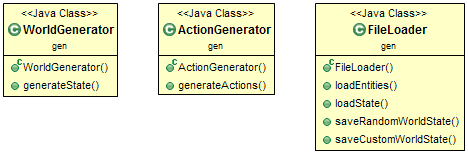
\includegraphics[scale=0.9]{img/gen.png}
\caption{Grafická reprezentácia balíčka gen.}
\label{fig:ch32}
\end{center}
\end{figure}
Grafickú reprezentáciu môžeme sledovať na obrázku 3.2. Tento diagram nie je veľmi zložitý, keďže tieto triedy sú od seba nezávislé. Ale majú spoločnú funkcionalitu a preto sú zaradené do tohto balíčka.
\subsection{Balíček goap}
Balíček goap bude pozostávať z tried, ktoré budú mať na starosti plánovanie akcií, teda príbehu a tiež aj hodnotenie naplánovaného príbehu.\par
Prvou triedou tohto balíčka bude trieda reprezentujúca akciu. Bude to abstraktná trieda a bude slúžiť ako predloha jednotlivým, konkrétnym akciám. Ďalej sa tu bude nachádzať trieda Planner. Táto trieda bude mať za úlohu naplánovať pomocou akcií príbeh, ktorý sa bude neskôr skúmať kvôli ohodnoteniu a následne sa bude dať zahrať. Keďže plánovanie by malo byť implementované pomocou grafového algoritmu, tak táto trieda bude obsahovať aj vnorenú triedu pre reprezentáciu vrcholu v grafe. Tento vrchol bude uchovávať štyri atribúty. Bude si uchovávať cenu, ktorou sme sa dostali do daného vrcholu, počet zatiaľ nevyriešených cieľov v tomto vrchole, stav, ktorý tento vrchol reprezentuje a nakoniec akciu, ktorou sme sa dostali do tohto vrcholu. Taktiež si bude uchovávať referenciu na svojho rodiča, aby sme po skončení plánovacieho procesu vedeli, nájsť cestu od počiatočného stavu k cieľovému. Posledná trieda nachádzajúca sa v tomto balíčku bude PlanEvaluator, ktorý po naplánovaní príbehu plánovačom, ohodnotí daný príbeh podľa určených kritérii. Grafický model môžeme vidieť na obrázku 3.3.
\begin{figure}[H] 
\begin{center}
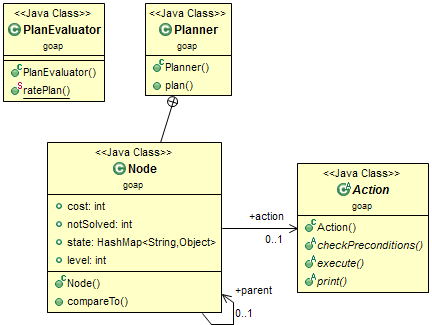
\includegraphics[scale=0.9]{img/goap.png}
\caption{Grafická reprezentácia balíčka goap.}
\label{fig:ch33}
\end{center}
\end{figure}
\subsection{Balíček game}
V tomto balíčku budeme uchovávať triedy, súvisiace priamo s hracím prostredím aplikácie. Prvú ktorú spomenime je trieda GameWorld. Trieda GameWorld bude uchovávať všetky možné informácie o hernom svete. Bude si pamätať všetky načítané objeky daného sveta aj akcie vygenerované tomuto svetu. Ďalej bude obsahovať reprezentáciu pre svoj svet a aj cieľ, ktorý v tomto svete chceme dosiahnuť. Navyše, bude uchovávať naplánovanú postupnosť akcií, hodnotenie príbehu pre daný svet a aj hodnotu semiačka, ktorá bola použitá na generovanie tohto sveta. Taktiež, bude obsahovať referencie na triedy z balíčka gen, pomocou, ktorých sa svet, ktorý táto trieda reprezentuje, vygeneruje. Trieda si bude uchovávať aj referenciu na plánovač z balíčka goap, ktorý využie na vytvorenie príbehu pre daný svet. Druhou triedou bude trieda GameView. Táto trieda bude sporsdredkúvať odozvu používateľovi počas hrania niektorého z príbehov. Bude využívaná na opis herného sveta a vlastnosti hrdinu, ktorého bude používateľ stvárnovať vo svete. Tiež ju použijeme na uvedenie používateľa do deja a na zobrazenie každého ťahu, ktorý sa vykoná. Ak sa používateľ dostane do cieľového stavu hracieho sveta, tak táto trieda mu sprosdredkuje koniec príbehu. Ďaľšou triedou tohto balíčka by mala byt trieda GameController. Táto sa využije na ovládanie aplikácie. Bude teda poskytovať prepojenie medzi našimi troma hlavnými funkcionalitami. Umožní používateľovi vybrať si z týchto troch hlavných funkcionalít a spustí vybranú časť aplikácie. Navyše bude fungovať aj ako hrací engine. Posledná trieda v tomto balíčku bude trieda Game, ktorá iba spustí GameController a prípadne odchytí výnikmy a poskytne spätnú väzbu používateľovi ak sa vyskytne nejaký problém. Na obrázku 3.4 uvádzame grafickú reprezentáciu týchto tried.
\begin{figure}[H] 
\begin{center}
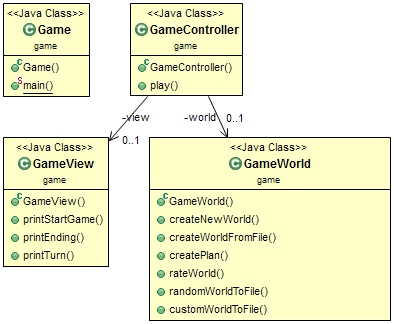
\includegraphics[scale=0.9]{img/game.png}
\caption{Grafická reprezentácia balíčka game.}
\label{fig:ch34}
\end{center}
\end{figure}
\section{Reprezentácia herného sveta}
Kým sa dostaneme ku generovaniu sveta musíme najprv navrhnúť reprezentaciu herného sveta. Herný svet by mal byť reprezentovaný, niečim ako interpretáciou predikátov. Teda v aplikácii by sme mali definovavé rôzne predikáty a ich hodnoty by mali tvoriť herný svet. Napríklad by sme mali predikát Place(X), kde X reprezentuje niektorý z herných objektov a tento predikát by nám vrátil hodnotu, kde sa v hernom svete tento objekt nachádza. Podobne by sme mohli mať predikát CanTravelFromTo(X,Y). Tento predikát by hovoril o tom, či existuje cesta z miesta X do miesta Y. A takýmito rôznymi ďaľšími predikátmi, vytvoríme celý náš herný svet.\par
Ako je spomenuté v špecifikácii, mali by sme vedieť túto reprezentáciu zapísať do súboru vo formáte ľahko čitateľnom človeku. Čiže naša aplikácia prejde postupne cez všetky hodnoty predikátov, ktoré sú pravdivé v danej reprezentácii sveta a zapíše ich do textového súboru. Formát súboru by mal vyzerať podobne ako popisuje obrázok 3.5.
\begin{figure}[H] 
\begin{center}
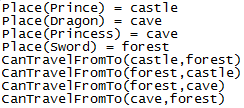
\includegraphics[scale=1.0]{img/dosuboru.png}
\caption{Ukážka formátovania reprezentácie herného sveta v súbore.}
\label{fig:ch35}
\end{center}
\end{figure}
Opačným postupom by sme mali vedieť získať reprezentáciu sveta zo súboru do našej aplikácie. Teda rozparsujeme daný textový súbor a jednotlivými hodnotami naplníme hodnoty predikátov v aplikácii s ktorými potom budeme ďalej pracovať.
\section{Reprezentácia akcií}
Akcie budú reprezentované ako jednotlivé triedy v aplikácii. Budú mať za úlohu meniť hodnoty predikátov a tým teda budú môcť ovplyvnovať herný svet. Pre vhodnú reprezentáciu akcií bude potrebné aby obsahovali dve funkcie.\par
Prvá, ktorá zistí, či sa daná akcia môže vykonať v konkrétnom stave herného sveta. Druhou bude funkcia, ktorá zmení hodnoty v reprezentácii sveta podľa konkrétnej akcie. Túto reprezentáciu akcií budeme využívať pri plánovaní príbehu aj pri samotnom hraní.\par
Taká najjednoduchšia by mala byť akcia Move(Who, Where), ktorá teda zistí kde sa nachádza objekt Who pomocou hodnoty z predikátu Place(Who), potom sa pozrie či hodnota predikátu CanTravelFromTo(Place(Who),Where) je nastavená ako pravdivá. Toto je súšasťou prvej spomínanej funkcie, teda akcia Move zistí či daný objekt Who je možné presunúť na miesto Where. Ak áno tak sa použije druhá zo spomínaných funkcií akcie, ktorá zmení hodnotu predikátu Place(Who) na hodnotu Where.
\section{Generovanie sveta a akcií}
Už sme popísali reprezentáciu herného sveta aj akcií, tak v tejto časti podrobnejšie uvedieme ako budeme generovať herný svet a akcie.\par
Na generovanie herného sveta využijeme pseudo-náhodný generátor hodnôt z Javy. Za pomoci načítaných herných objektov zo súborov a podľa hodnoty, ktorú dostaneme z generátora hodnôt, postupne popriradzujeme hodnoty predikátom, ktoré tvoria herný svet. Teda ak by sme zo súboru mali načítané entity Prince, Princess, Dragon, Sword, tak za pomoci generátora náhodných priradíme predikátom Place(Prince), Place(Princess), Place(Dragon), Place(Sword) hodnotu prislúchajúcu jednému z načítaných herných miest. Týmto spôsobom naplníme hodnoty všetkým predikátom našej aplikácie pričom generátor náhodných hodôt nám vždy vyberie konkrétnu hodnotu predikátu.\par
Ako už bolo spomenuté, pri generovaní využívame pseudo-náhodný generátor hodnôt, ktorý generuje hodnoty podľa nejakej inicializačnej hodnoty. Táto hodnota sa po vygenerovaní sveta a pred začiatkom hry zobrazí používateľovi. Používateľ bude mať možnosť pred generovaním sveta nastaviť túto hodnotu a tým zreprodukovať predošlé vygenerované svety.\par
Generovanie akcií bude spravené jednoduchým spôsobom. Každá akcia sa vygeneruje pre všetky možné kombinácie načítaných objektov zo súboru. Napríklad teda budeme mať, toľko inšatncií akcie Move(Who, Where) koľko kombinácii dvojíc Who a Where bude načítané zo súboru. Dôvodom je potencionálna možnoť presunúť, každý objekt Who na hociktoré z miest Where. 
\section{Plánovanie príbehu}
Pri plánovaní budeme využívať našu reprezentáciu sveta a akcií na vygenerovanie postupnosti akcií, ktoré nás dostanú z počiatočného stavu do cieľového. Na plánovanie využijeme algoritmus, ktorý je popísany vo východiskovej kapitole v časti o cieľovo orientovanom plánovaní akcii.\par
Aby bolo toto možné tak, každá akcia bude mať svoju hodnotu založenú na zaujímavosti danej akcie. Túto hodnotu použije algoritmus na ocenenie hrán grafu. Hodnotiť budeme spôsobom, čím menšia hodnota tým lepšie. Napríklad akcia na premiestňovanie postáv bude mať horšiu hodnotu ako akcia na zdvihnutie predmetu a tá bude mať zase horšiu hodnotu ako akcia na súboj dvoch postáv, keďže toto nám príde zaujímavejšie. Táto hodnota sa bude kumulovať v triede ktorá reprezentuje vrchol grafu. Vrchol grafu bude teda obsahovať súčet zaujímavostných hodôt svojich rodičov a seba.\par
Po zistení, že sme v prehľadávaní dostali do cieľového stavu, teda že sme našli konkrétny plán, si zapamäťáme vrchol, ktorý reprezentuje tento cieľový stav a pokračujeme v prehľadávaní až kým nenájdeme všetký možné plány daného sveta. Keď prehľadávanie skončí, tak prejdeme všetkými zapamätanými vrcholmi, ktoré sme našli a vyberieme ten s najmenšou cenou, pretože reprezentuje najzaujímavejší príbeh. V tomto vrchole využijeme jeho referenciu na rodiča a príbeh zrekonštruujeme tak ako má byť od začiatku do konca.
\section{Hodnotenie príbehu}
Hodotiť príbeh budeme formou analyzovania dynamiky príbehu. Podľa našej hypotézi by mal príbeh mať rovnomerne rozložené zaujímavé akcie a menej zaujímave akcie, tak aby sa v príbehu nevyskytovala nejaká jednotvárna časť. Budeme teda sledovať štruktúru príbehu a aj poradie akcíí v príbehu.\par
Každý príbeh bude mať svoje hodnotenie v číselnej forme a keď sa vyskytne nejaká vlastnosť v príbehu, ktorú onzačíme ako nezaujímavú tak z daného hodnotenia odpočítame príslušnú hodnotu. Budeme sledovať napríklad či sa daná akcia v príbehu neopakuje veľa kráť za sebou, či sú v príbehu využité všetky možné akcie, následnosť jednotlivých zaujímavejších akcií, náväznoť akcií teda či sú akcie, ktoré na seba naväzujú, prerušené inou akciou alebo nie, akou akciou začína príbeh a pod. Po tomto ohodnotení sa hodnota priradí k danému svetu, aby sa neskôr mohol vybrať ten najzaujímavejší, ktorý sa poskytne používateľovi.
\section{Ovládanie aplikácie}
Aplikácia sa bude ovládať pomocou príkazov do konzoli. Používateľ vždy dostane na výber zoznam príkazov, ktoré môže v danom štádiu aplikácie použiť. V niektorých štádiách bude aplikácia očakávať aj vstupné údaje od používateľa. Po zadaní príkazu aplikácia vykoná daný príkaz a poskytne používateľovi ďaľšiu sadu príkazov alebo skončí.
\section{Herná časť aplikácie}
Samotná hra bude taktiež reprezentovná pomocou konzoli, koniec koncov ide o textovú hru. Po vygenerovaní alebo načítaní sveta aplikácia vypíše na konzolu semiačko podľa, ktorého bol svet vygenerovaný a uvedie používateľa do deja. Po úvode sa už vypíše samotný hrací ťah. Aplikácia poskytne používateľovi na konzolu lokáciu v ktorej sa hrdina nachádza. Budú poskytnuté aj informácie čo sa nachádza v danej lokalite, teda či sú tam nejaké objekty alebo iné herné entity s ktorými by hrdina mohol interagovať. Daľším výpisom budú pozície na ktoré hráč môže posunúť svojho hrdinu. Tiež sa vypíše aj hrdinov inventár. Na koniec sa používateľovi vypíše zoznam akcií, ktoré môže hrdina v danej lokácii vykonať. Potom ako používateľ zadá nejakú akciu na vykonanie, tak sa tento proces zopakuje s tým, že sa údaje aktualizujú vzhľadom na akciu, ktorú používateľ vykonal. Ak sa vykoná cieľová akcia, tak hra vypíše koniec príbehu a aplikácia skončí.


